\documentclass{article}
\usepackage[T1]{fontenc}
\usepackage[utf8]{inputenc}
\usepackage{lmodern}
\usepackage[ngerman]{babel}
\usepackage{amsmath, amssymb}
\usepackage{array}
\usepackage{phonetic} % for reversed D
\usepackage{wasysym}  % for the notes
\usepackage{tikz, tikzsymbols}
\usepackage{xcolor}


\usetikzlibrary{arrows,automata,fit}
\setlength\parindent{0pt}

    
\begin{document}

\begin{center}
  \Large{Informatik \revD: Übungsblatt 8}

  \large{Sebastian Höffner, Andrea Suckro}
\end{center}



\section*{Aufgabe 8.1}
Idee: Da wir beim Start der Maschine schon ganz links also am MSB des Eingabewortes stehen, müssen wir danach nur noch alle danach kommenden Zeichen durch a ersetzen, um auf den Log zu kommen (wir löschen also die erste 1 da $\log_2(10_2) = 1$). Unser Automat behandelt auch noch den Fall, dass das Eingabewort mit beliebig vielen Nullen beginnt. Wenn das Wort nur Nullen enthält soll die Maschine in eine Endlosschleife verfallen, da $\log(0)$ nicht definiert ist.
%Automat für die TM
\begin{center}
\begin{tikzpicture}[->, auto, node distance=2cm]
  \node[state,initial] (S)      {};
  \node[state]         (A) [right of=S] {};
  \node[state]         (B) [right of=A] {};
  \node[state]         (C) [right of=B] {};
 
  \path (S) edge                            node {$1/\square,R$}       (A)
            edge [loop below, align=center] node {$0/\square,R$ \\ $\square/\square,R$} (S) %wir ersetzen die erste 1 
        (A) edge [loop below, align=center] node {$0/a,R$ \\ $1/a,R$}  (A) %wir ersetzen alle Zeichen mit a
            edge                            node {$\square/\square,L$} (B) %am Ende gehen wir nach links
        (B) edge [loop below]               node {$a/a,L$}             (B) %hier gehen wir alle as zurück
            edge                            node {$\square/\square,R$} (C) %damit kommen wir an den Anfang des Wortes
        ;
\end{tikzpicture}
\end{center}



\section*{Aufgabe 8.2}
\subsection*{a) Turingmaschine für $\alpha$ ungerade}
Meine Idee dazu lautet wie folgt: ich ersetze das erste $\alpha$ mit S. Dann gehe ich bis zum Ende, lasse ein Kästchen als Trennung stehen und schreibe 2 $\alpha$. Dann gehe ich bis vor das letzte S zurück und wiederhole alles. Am Schluss hat man so für jedes $\alpha$ hinten 2 $\alpha$s geschrieben. Jetzt ersetzt man noch das Kästchen in der Mitte (das ist die $+1$ in der Formel) und ersetzt alle S wieder durch $\alpha$. Damit hat man insgesammt: $\alpha+1+2\cdot \alpha = 3\alpha +1$.

\begin{center}
\begin{tikzpicture}[->, auto, node distance=2cm]
  \node[state,initial] (S)      {};
  \node[state]         (A) [right of=S] {};
  \node[state]         (B) [right of=A] {};
  \node[state]         (C) [right of=B] {};
  \node[state]         (D) [right of=C] {};
  \node[state]         (E) [below of=C] {};
  \node[state]         (F) [below of=A] {};
  \node[state]         (G) [below left of=E] {};
  \node[state]         (H) [below of=G] {};
  \node[state]         (I) [left of=H]  {};
   
  \path (S) edge                            node {$\alpha/S,R$}        (A) %das erste alpha durch S ersetzen
        (A) edge [loop above, align=center] node {$\alpha/\alpha,R$}   (A)
            edge                            node {$\square/\square,R$} (B) 
        (B) edge [loop above]               node {$\alpha/\alpha,R$}   (B) 
            edge                            node {$\square/\alpha,R$}  (C)
        (C) edge                            node {$\square/\alpha,L$}  (D)
        (D) edge [loop above]               node {$\alpha/\alpha,L$}   (D)
            edge                            node {$\square/\square,L$} (E)
        (E) edge                            node {$\alpha/\alpha,L$}   (F)
            edge                            node {$S/S,R$}             (G)
        (F) edge [loop below]               node {$\alpha/\alpha,L$}   (F)
            edge                            node {$S/S,R$}             (S)
        (G) edge                            node {$\square/\alpha,L$}  (H)
        (H) edge [loop right]               node {$S/\alpha,L$}        (H)
        (H) edge                            node {$\square/\square,R$} (I)
        ;
\end{tikzpicture}
\end{center}


\subsection*{b) Generelles Vorgehen}
Wir müssen zunächst rausfinden ob die Zahl gerade oder ungerade ist. Das geht relativ leicht über folgenden Automaten:
\begin{center}
\begin{tikzpicture}[->, auto, node distance=3cm]
  \node[state,initial] (A) {};
  \node[state]         (B) [right of=A] {};
  \node[state]         (C) [below of=B] {};
  \node[state]         (D) [below of=A] {};
   
  \path (A) edge [bend right]   node {$\alpha/\alpha,R$}  (B)
            edge                node {$\square/\square,L$}(D) 
        (B) edge [bend right]   node {$\alpha/\alpha,R$}  (A)
            edge                node {$\square/\square,L$}(C)
        (C) edge [loop right]   node {$\alpha/\alpha,L$}  (C)
        (D) edge [loop left]    node {$\alpha/\alpha,L$}  (D)
        ;
\end{tikzpicture}
\end{center}
Von dessen Enden können wir in den passenden Automaten verzweigen. Für ungerade (rechts) haben wir in a) schon den Automaten generiert. Der Automat zur Halbierung der Zahl kann ähnlich konstruiert werden. Dafür ersetzen wir die beiden ersten $\alpha$ durch ein S, gehen nach rechts durch all die anderen $\alpha$ bis zum Kästchen und schreiben hinter das Kästchen ein $\alpha$. Dann gehen wir zu dem Kästchen zurück. Überprüfen ob neben dem Kästchen noch ein $\alpha$ steht und gehen bis zu dem letzten S. Dann ersetzen wir wieder 2 $\alpha$ mit S, gehen bis zu dem Kästchen, gehen von da durch alle $\alpha$ und schreiben ein neues hinten dran. Irgendwann wird der Punkt kommen wo wir nach dem Kästchen direkt ein S stehen haben. Dann können wir nach links gehen und alle S durch Kästchen ersetzen. Dann (wenn wir an Kästchen links angekommen sind) gehen wir wieder nach rechts bis wir das erste $\alpha$ finden und sind fertig.

\section*{Aufgabe 8.3}
\emph{Noch nicht sinnvoll formuliert, nur vage Ideen}

Die beiden Definitionen sehen auf den ersten Blick identisch aus. Insbesondere wirkt eigentlich gerade die zweite nicht mächtiger (keine Erwähnung der Randsymbole). 

Auf den zweiten Blick kann ich höchstens sagen, dass die zweite Definition erlaubt, auch woanders hin zu schreiben.
D.h. wenn mein Band n Eingabesymbole hat, kann ich an n beliebige Stellen schreiben, nicht nur dort, wo auch die Eingabe ist. Man könnte dann argumentieren, dass sie mächtiger erscheint, weil ich das Eingabewort unangetastet lassen kann und immer wieder lesen kann -- Aber da wir ja in der VL gelernt haben, dass man beliebig viele States von beliebig vielen Bändern zusammen fassen kann als einen State, können wir eine Umformung finden von der ersten Definition in die zweite und umgekehrt, wodurch sie äquivalent sind.


\section*{Aufgabe 8.4}
Die Idee ist hier bei beiden Programmen so lange von beiden Zahlen 1 abzuziehen bis die erste 0 erreicht. Die Zahl die als erstes 0 erreicht ist das Minimum und wird ausgegeben.
\subsection*{a) GOTO-Programm für $min(x_1,x_2)$}
%Basti- wenn dir eine bessere Sache für den Code einfällt, dann gerne los :)
\begin{verbatim}
    x4 = x1
    x5 = x2
L1: x4 = x4-1
    x5 = x5-1
    if x4 != 0
      goto L2
    x3 = x1
    halt
L2: if x5 != 0
      goto L1
    x3 = x2
    halt
\end{verbatim}
Alternative:
\begin{verbatim}
    x3 = 0
    x4 = x1
    x5 = x2
L1: x4 = x4 - 1
    x5 = x5 - 1
    x3 = x3 + 1
    if x4 != 0 goto L2
    halt
L2: if x5 != 0 goto L1
    halt
\end{verbatim}
\subsection*{b) WHILE-Programm für $min(x_1,x_2)$}
\begin{verbatim}
x4 = 1;
x5 = x1;
x6 = x2;
while(x4 != 0){
  x5 = x5 - 1;
  x6 = x6 - 1;
  if(x5 != 0){}
  else{
    x3 = x1;
    x4 = 0;
  }
  if(x6 != 0){}
  else{
    x3 = x2;
    x4 = 0;
  }
}
\end{verbatim}
Alternative:
\begin{verbatim}
x3 = 0;
x4 = x1;
x5 = x2;
while(x4 != 0) {
  x4 = x4 - 1;
  x5 = x5 - 1;
  x3 = x3 + 1;
  if(x5 != 0) {}
  else {
    x4 = 0;
  }
}
\end{verbatim}
\section*{Aufgabe 8.5}

Juhu -- Frei-Punkte $:)$




\section*{Aufgabe 8.6}
\begin{figure}[!h]
  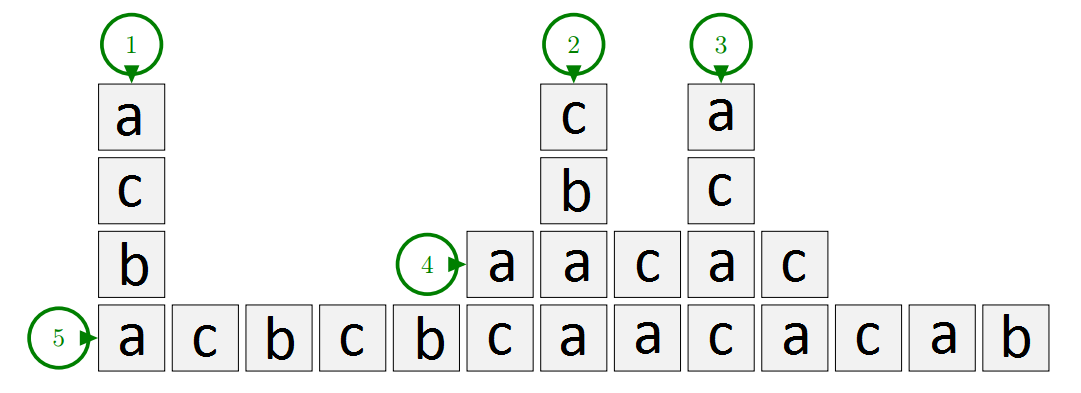
\includegraphics[scale=0.4]{crossword.png}
\end{figure}

\end{document}
